\documentclass[12pt]{article}


\usepackage{todonotes}
\usepackage{tikz}
\usetikzlibrary{shapes, arrows, calc, math}
\usepackage{subfig}
\usepackage{amsmath}
\begin{document}
\section{Definitions}
Vectors are bold $(\mathbf{v})$, and unit vectors are bold with hats $(\mathbf{\hat{v}})$.\\
The cross product in 2 dimensions is:
\begin{equation}
	\label{eq:cross_prod_2d}
	\mathbf{a}\times \mathbf{b} = a_xb_y - b_x a_y
\end{equation}
The anti-clockwise (left) and clockwise (right) perpendicular vector to $\mathbf u$ are given by:
\begin{equation}
	\mathbf{\bar u_L} = \left(\begin{matrix}
		-u_y\\
		u_x
\end{matrix}\right)
\end{equation}
\begin{equation}
	\mathbf{\bar u_R} = \left(\begin{matrix}
		u_y\\
		-u_x
\end{matrix}\right)
\end{equation}
\section{Collisions}
\subsection{Collision of circle and boundary line}
We have a static boundary line and a circle, which is intersecting it. We want to work out where the circle would be had it elastically bounced off the line instead of intersecting. The circle is at position $\mathbf{a}$, has a radius $R$ and a velocity vector $\mathbf{v}$. The circle's path tangent has the equation $\mathbf{r}(\lambda) = \lambda \mathbf{v} + \mathbf{a}$.
The boundary line contains the point with position vector $\mathbf{b}$ and is in direction $\mathbf{\hat{u}}$, so has the equation $\mathbf{l}(\gamma) = \gamma \mathbf{\hat{u}} + \mathbf{b}$. We want to find the point $\mathbf{w}$ along the line $\mathbf r(\lambda)$ where the circle is just touching the line. 
The displacement vector from the circle's current position to the intersection point, $\mathbf{d} = \mathbf{a}-\mathbf{w}$ is then inverted through the vector $\mathbf{\hat{u}}$ and the resultant vector, $\mathbf{\tilde d}$ is added to $\mathbf{w}$ to give the reflected position.
\\ 
This process is shown in figure \ref{fig:line_circle_collision}
\begin{figure}
	\centering
	\subfloat{
	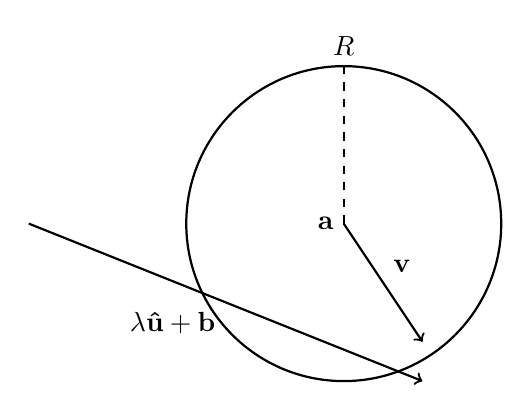
\begin{tikzpicture}
		\draw[thick] (4, 0) circle (2) {};
		\draw[dashed, thick] (4, 0) node[anchor=east] {$\mathbf{a}$} to (4, 2) node[anchor=south] {$R$};
		\draw[thick, ->] (4, 0) to node[auto] {$\mathbf{v}$} (5, -1.5) {};
		\draw[->, thick] (0, 0) to node[auto, swap] {$\lambda\mathbf{\hat{u}}+\mathbf{b}$} (5, -2) {};
	\end{tikzpicture}
}\qquad
	\subfloat{
	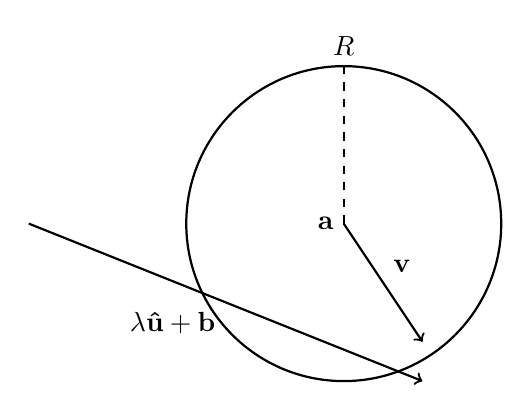
\begin{tikzpicture}
		\draw[thick] (4, 0) circle (2) {};
		\draw[dashed, thick] (4, 0) node[anchor=east] {$\mathbf{a}$} to (4, 2) node[anchor=south] {$R$};
		\draw[thick, ->] (4, 0) to node[auto] {$\mathbf{v}$} (5, -1.5) {};
		\draw[->, thick] (0, 0) to node[auto, swap] {$\lambda\mathbf{\hat{u}}+\mathbf{b}$} (5, -2) {};
	\end{tikzpicture}
}\qquad
	\caption{Hello}
	\label{fig:line_circle_collision}
\end{figure}
\\
First we want to find the position where the centre of the circle touches the line, $\mathbf{p}$.
\begin{equation}
	\begin{split}
		\mathbf{r}(\lambda) &= \mathbf{l}(\gamma) \\
		\left(\begin{matrix}\lambda v_x+a_x \\ \lambda v_y+a_y\end{matrix}\right) &= 
		\left(\begin{matrix}\gamma \hat u_x+b_x \\ \gamma \hat u_y+b_y\end{matrix}\right)
		\\
		\gamma&= \frac{\lambda v_x + a_x - b_x}{\hat u_x}\\
		\lambda&= \frac{\gamma \hat u_y + b_y - a_y}{v_y}\\
		\lambda - \frac{\lambda v_x \hat u_y}{\hat u_x v_y} &= \frac{(\mathbf{a}-\mathbf{b})\times \mathbf{ \hat u}}{\hat u_xv_y}\\
		\lambda &= \frac{(\mathbf{a}-\mathbf{b})\times \mathbf{ \hat u}}{\mathbf{\hat u} \times \mathbf{v}}
	\end{split}
\end{equation}
And so: 
\begin{equation}
	\mathbf p = \frac{(\mathbf{a}-\mathbf{b})\times \mathbf{ \hat u}}{\mathbf{\hat u} \times \mathbf{v}} \mathbf{v} + \mathbf{a}
\end{equation}
We now calculate from this point the point on the line $\mathbf r(\lambda)$ which is the distance $R$ along $\mathbf{\bar u}_{L,R}$
\begin{equation}
\lambda_{ L, R} = \frac{R}{\mathbf v \cdot \mathbf{\bar u}_{L,R}}
\end{equation}
And now we can work out the two points along the line $\mathbf r(\lambda)$ where the circle is just touching the line $\mathbf l(\gamma)$:
\begin{equation}
\mathbf{w}_{\pm}=\mathbf{w}_{L,R} = \frac{R}{\mathbf v \cdot \mathbf{\bar u}_{L,R}} \mathbf v + \mathbf p = \frac{(\mathbf a - \mathbf b) \times \mathbf{\hat u}\pm R}{\mathbf{\hat u}\times \mathbf{v}} \mathbf v + \mathbf a
\end{equation}
We then have the displacement vector $\mathbf d_{\pm} = \mathbf a - \mathbf w_{\pm}$ which we need to flip around the vector $\mathbf {\hat u}$. We perform this with the rotated parity operator P, with a rotation of the angle $\theta$ between the x-axis and $\mathbf {\hat u}$:
\begin{equation}
	\begin{split}
		P &= R^T P_x R\\
		   &= \left(\begin{matrix}\cos \theta & \sin \theta \\ -\sin \theta & \cos \theta\end{matrix}\right)
		\left(\begin{matrix}1 & 0 \\ 0 & -1\end{matrix}\right)
		\left(\begin{matrix}\cos \theta&  -\sin \theta \\ \sin\theta &\cos\theta \end{matrix}\right) \\
					       &= \left(\begin{matrix} \cos\theta & -\sin\theta \\ -\sin \theta & -\cos \theta \end{matrix}\right)\left(\begin{matrix}\cos \theta&  -\sin \theta \\ \sin\theta &\cos\theta \end{matrix}\right)\\
					       &= \left(\begin{matrix} \cos^2\theta-\sin^2\theta & -2\sin\theta\cos\theta \\ -2\sin \theta\cos\theta & \sin^2 \theta-\cos^2\theta \end{matrix}\right)
	\end{split}
\end{equation}
We can write these angles using the cross product and the dot product:
\begin{align}
	\mathbf{\hat u}\times \mathbf{\hat x} = \sin \theta && \mathbf{\hat u} \cdot \mathbf{\hat x} = \cos \theta
\end{align}
\begin{equation}
	P = \left(\begin{matrix}(\mathbf{\hat u}\cdot \mathbf{\hat x})^2-(\mathbf{\hat u}\times \mathbf{\hat x})^2 & -2(\mathbf{\hat u}\times\mathbf{\hat x})(\mathbf{\hat u}\cdot\mathbf{\hat x}) \\
	-2(\mathbf{\hat u}\times\mathbf{\hat x})(\mathbf{\hat u}\cdot\mathbf{\hat x}) & 
	(\mathbf{\hat u}\times \mathbf{\hat x})^2 - (\mathbf{\hat u}\cdot \mathbf{\hat x})^2\end{matrix}\right)
\end{equation}
Which can be simplified using the components of $\mathbf{\hat u}$ and $\mathbf{\hat x}$.
\begin{equation}
	P = \left(\begin{matrix}
		u_x^2 - u_y^2 & 2 u_x u_y \\
		2 u_x u_y & u_y^2-u_x^2
	\end{matrix}\right)
\end{equation}
And we have the new, reflected position: 
\begin{equation}
	\mathbf x_{\pm}=  \mathbf a + \frac{(\mathbf a- \mathbf  b)\times \mathbf{\hat u} \pm R}{\mathbf{\hat u} \times \mathbf v}
(I - P) \mathbf v
\end{equation}
\begin{equation}
	I-P = \left(\begin{matrix}
		2u_y^2 & -2u_xu_y \\
		-2u_xu_y& 2u_x^2
	\end{matrix}\right) 
\end{equation}
\begin{equation}
	\mathbf x_{\pm}=  \mathbf a + \frac{(\mathbf a- \mathbf  b)\times \mathbf{\hat u} \pm R}{\mathbf{\hat u} \times \mathbf v}
(I - P) \mathbf v
\end{equation}

\begin{equation}
	\mathbf x_{\pm}=  \mathbf a + 2((\mathbf a- \mathbf  b)\times \mathbf{\hat u} \pm R) \mathbf{\bar u}_{L}
\end{equation}

\end{document}
